\section{Workloads}
\label{research-design-and-methodology:workloads}

Each workload that the configurations execute is mapped to the access or index mechanism it is designed to stress, so that a difference between configurations traces to that mechanism rather than to the workload as a whole. The experimental design fixed which factor each research question varies, and which conditions are held constant. Rather than covering the query language, the workloads exercise the two structural axes established in the background. The first is the divide between formats a client can read in part and formats that require a full scan, identified in Section~\ref{background:spatial-data-formats-and-storage-models:summary} as the primary axis for interpreting read performance. The second is the distributed query lifecycle of Section~\ref{background:distributed-spatial-processing:the-lifecycle-of-a-distributed-spatial-query}, whose planning, shuffle, and collection phases determine where a distributed engine spends time and bytes.

\subsection{Workload taxonomy}
\label{research-design-and-methodology:workloads:workload-taxonomy}

The workloads fall into two families, one per the first two research questions. \acrshort{rq}1 uses three single-machine query patterns over a single input: a point-in-polygon test, a $k$-nearest-neighbor search, and a bounding-box range filter. \acrshort{rq}2 uses a single national-scale spatial join between two inputs, run on the distributed engine and on the single-node engines that serve as its reference. The single-machine patterns isolate how a format and engine read and prune one dataset, whereas the join exercises the cross-input coordination that only a distributed lifecycle incurs.

Each pattern stresses a distinct mechanism. The point-in-polygon test resolves an intersection predicate, the predicate class for which both single-node engines consult an R-tree (Section~\ref{background:spatial-data-formats-and-storage-models:full-database-engines}), so it measures how effectively that index narrows the candidate set. The $k$-nearest-neighbor search orders features by distance to a fixed point. Distance ordering gains no help from the spatial index unless a bounding-box predicate is also supplied (Section~\ref{background:spatial-data-formats-and-storage-models:full-database-engines}), so the search probes the cost of a predicate the index does not directly serve. The bounding-box range filter is the pattern that range-request formats are built for: block-level pruning against per-row-group statistics and the GeoParquet bounding-box covering answers it (Section~\ref{background:geometry-and-indexing:spatial-indexing}), while the format-level predicate and projection pushdown of Section~\ref{background:spatial-data-formats-and-storage-models:file-formats} govern how many bytes leave storage. The spatial join is a wide operation that crosses a stage boundary and resolves through either broadcast or partitioned execution (Section~\ref{background:distributed-spatial-processing:distributed-spatial-operations}). On this workload the distributed lifecycle of Section~\ref{background:distributed-spatial-processing:the-lifecycle-of-a-distributed-spatial-query} either repays its coordination cost or does not.

\subsection{Workload definitions}
\label{research-design-and-methodology:workloads:workload-definitions}

Each single-machine workload is defined by three elements: the spatial predicate it evaluates, the fixed reference geometry against which the predicate is tested, and the shape of the result it returns. The point-in-polygon workload tests a fixed query point against the building polygons and returns the polygon or polygons containing it. The $k$-nearest-neighbor workload ranks the buildings by distance to a fixed query point and returns the $k$ closest buildings. The bounding-box workload applies a fixed rectangular window and returns every building whose geometry intersects it; the window is sized to a fixed selectivity, so the fraction of the dataset returned stays constant across tiers. Figure~\ref{fig:single-machine-query-definitions} shows the three patterns geometrically against a shared building set. Because the reference geometry and the returned fraction are held constant across configurations, a difference in time or transferred bytes can be attributed to the format and engine rather than to how much data each query happened to touch.

\begin{figure}[H]
    \centering
    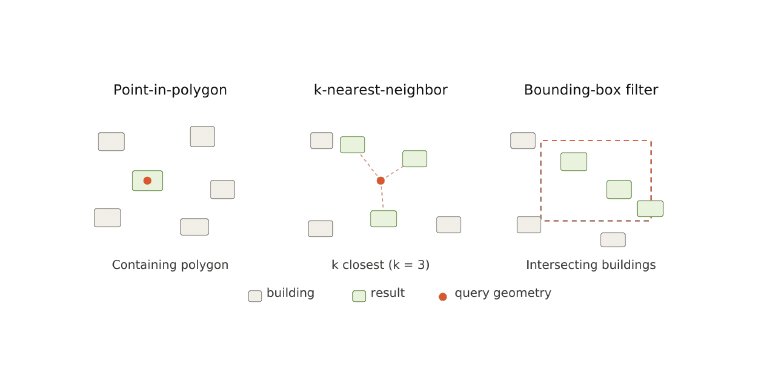
\includegraphics[width=0.95\textwidth]{Chapters/04-research-design-and-methodology/sub-chapters/figures/04-single-machine-query-definitions.png}
    \caption[Single-machine query patterns.]{The three single-machine query patterns, each evaluated against the same building set, with query geometry shown in coral and result features in green. (a) Point-in-polygon returns the polygon containing a fixed query point. (b) $k$-nearest-neighbor returns the $k$ buildings closest to a fixed query point, here $k = 3$. (c) Bounding-box filter returns every building whose geometry intersects a fixed rectangular window.}
    \label{fig:single-machine-query-definitions}
\end{figure}

The \acrshort{rq}2 workload is a spatial join between Norwegian municipal boundaries and the building dataset, evaluated with an intersection predicate and grouped per municipality, so that each building is associated with the municipality whose boundary contains it. The single-machine patterns run at small and large dataset tiers, whereas the join runs at small, medium, and large tiers to trace its scaling behavior. The concrete record counts and the data layer that realizes each tier are described in Chapter~\ref{ch:system-architecture-and-implementation}. Table~\ref{tab:workload-matrix} summarizes each workload, its predicate, the configurations that execute it, and the tiers at which it is run.

\begin{table}[H]
    \centering
    \footnotesize
    \setlength{\tabcolsep}{6pt}
    \renewcommand{\arraystretch}{1.2}
    \begin{tabularx}{\textwidth}{@{}l >{\raggedright\arraybackslash}X >{\raggedright\arraybackslash}X l@{}}
        \toprule
        \textbf{Workload} & \textbf{Predicate} & \textbf{Configurations} & \textbf{Tiers} \\
        \midrule
        Point-in-polygon     & \texttt{ST\_Contains} point probe              & DuckDB + GeoParquet, PostGIS, DuckDB + Shapefile, Sedona + GeoParquet & Small, large \\
        $k$-nearest-neighbor & Distance ordering (\texttt{ST\_Distance})      & DuckDB + GeoParquet, PostGIS, DuckDB + Shapefile, Sedona + GeoParquet & Small, large \\
        Bounding-box filter  & Rectangular window (\texttt{ST\_Intersects})   & DuckDB + GeoParquet, PostGIS, DuckDB + Shapefile, Sedona + GeoParquet & Small, large \\
        \midrule
        Spatial join         & \texttt{ST\_Intersects} join, per municipality & Sedona (broadcast, partitioned; 2--16 workers), PostGIS, DuckDB       & Small, medium, large \\
        \bottomrule
    \end{tabularx}
    \caption[Benchmark workloads.]{The benchmark workloads, the predicate each evaluates, the configurations that execute it, and the dataset tiers at which it is run.}
    \label{tab:workload-matrix}
\end{table}

\subsection{Iteration counts}
\label{research-design-and-methodology:workloads:iteration-counts}
Every workload runs as a sequence of warmup iterations followed by timed iterations, with the warmup results discarded, following the replication protocol of Section~\ref{research-design-and-methodology:overview-and-experimental-design:replication-and-randomization}. Warmup primes the state that would otherwise contaminate the first timed measurement: the operating-system page cache, the database connection and its query-plan cache, just-in-time-compiled code paths in the engine, and, on the distributed engine, executors that have already been allocated and read their input once. For high-frequency single-machine queries, the measured variance determines the number of timed iterations via a relative-precision sequential stopping rule of the kind introduced by \textcite{georges2007_statistically_rigorous_java_performance} for performance benchmarks. After each timed iteration, the framework recomputes a bootstrap 95\% confidence interval for the mean elapsed time \parencite{laaber2019_software_microbenchmarking_cloud} and stops once its half-width falls below 5\% of the mean. Four bounds constrain the rule: a ten-iteration floor and a sixty-second timed window that must both be cleared before stopping is permitted, a soft ceiling at the per-workload iteration budget, and a one-hour hard timeout. The confidence interval on the mean governs only when sampling stops, while the location summary reported for each cell remains the minimum rather than the mean. The sample size reported for each benchmark cell is therefore the achieved iteration count recorded in the run metadata, not the configured ceiling. Section~\ref{research-design-and-methodology:statistical-analysis} gives the statistical treatment of the resulting samples, covering the estimator, the uncertainty quantification, and how the iteration count feeds into it.

The national-scale join takes the other branch. Because it is long-running and low in variance, a variance-driven stopping rule would buy little, so the join uses a fixed count of five timed iterations preceded by a single warmup iteration. Each iteration holds a Databricks cluster for its full duration, so further iterations multiply cluster costs without a proportional gain in precision, and five was judged the point beyond which each additional iteration returned too little to justify its cost. The single warmup primes the engine before the timed iterations begin.